\chapter{绪论}
本章首先阐述了本课题的研究背景及现实意义,然后介绍国内外针对该问题的研究与进展。同时说明在实际应用中存在的问题和可进一步优化的方法。最后介绍本论文的整体组织结构。
\section{研究背景与意义}
近年来,以神经网络\upcite{alexnet2012}为代表的深度学习方法在图像处理、机器视觉、自然语言处理等诸多应用领域取得了巨大突破。自2012年AlexNet\upcite{alexnet2012}以绝对优势夺得ImageNet冠军后,神经网络逐渐得到学术界、工业界的广泛关注,开启了人工智能新篇章。随后各种性能更优、结构更复杂的网络如雨后春笋般层出不穷。如VGG、inception系列、resnet系列,denseNet等\upcite{vgg2014, inception2015, resnet2016, denselynet2017}。同时,鉴于卷积神经网络在图像分类领域的优异表现,业界将其应用到了目标检测、图像分割等领域。如fast rcnn系列\upcite{rcnn2014, fastrcnn2015, fasterrcnn2015}、yolo系列\upcite{yolo2016}、FPN\upcite{fpn2017}、R-FCN\upcite{rfcn2016}等。在自然语言处理领域,涌现出了一系列以循环神经网络为基础的深度学习方法,在机器翻译、文本分析、阅读理解等\upcite{gnmt2016, bert2018}问题上取得了显著进步,达到甚至超越人类水平。

因为神经网络参数量、计算量巨大,往往需要花费数天,乃至更长的时间。如最初的AlexNet\upcite{alexnet2012},需要5-6天训完。使得网络更新迭代设计周期变长,极大限制了科研人员的研究进度。随着网络结构复杂化迭代周期过长的问题尤为严重。分布式训练神经网络则能极大缩短训练周期,加速研究迭代、产品孵化等。同时,随着神经网络的不断发展以及社会对人工智能应用需求的提升,深度学习所需的数据量、网络模型也越来越大,单台计算机算力已经很难甚至无法满足其计算要求。为了减少神经网络的训练时间和适应不断增长的算力要求,分布式训练神经网络是必然选择。

本课题围绕着分布式训练神经网络的效率和精度进行展开,旨在保证网络精度前提下,提升分布式训练神经网络效率和分布式训练系统的可扩展性。本课题不仅能解决现今训练神经网络时间过长的问题, 更为今后单机场景下无法完成训练的神经网络提供了高效的训练方法。这对于现阶段和可预见未来都有重要实用价值,促进神经网络的发展,对人工智能的发展有深远意义。

\section{研究现状}
随着人工智能的快速发展,为提升训练效率,满足生产需求。业界已针对分布式深度学习系统进行了深入的研究。目前业界主流深度学习框架同时支持parameter servers和horovod进行分布式训练。如tensorflow,pytorch,mxnet等\upcite{tensorflow2016, torch2002, mxnet2015}均支持pamameter servers和horovod。在通信效率上,针对神经网络的训练特点,CMU邢波教授课题组提出了一系列经典有效的方法:WFBP,SFB等。其petuum系统也受到广泛关注。在训练精度上,业界针对大batch size训练提出了一系列更新算法,保证大batch size的训练精度。如facebook何恺明等\upcite{train1hour2017}就提出线性增大学习率的方法保证了在batch size达到8k时,和单机batch size等于256时一致的精度,使得大规模分布式训练神经网络成为可能。随后,伯克利尤洋等提出LARS算法\upcite{train24min2017},在保证精度的情况下,进一步将batch size扩大到32k;紧接着Google Brain提出动态调整batch size的方法\upcite{dontdecay2018}将batch size提升到64k。
\subsection{分布式通信框架介绍}
目前主流深度学习框架均支持parameter servers和horovod。parameter servers最早由smola教授提出,最终由其学生李沐实现\upcite{ps2014}。其提供同步、异步、半异步的更新方式。因其灵活的更新方式和良好的性能得到业界广泛认可。参数服务器通过key-value键值对来管理参数。通常情况下,参数服务器是以去中心化的形式分散在多个节点,各个节点负责部分数据。其通信架构如图~\ref{fig:ps_comm_pattern}所示。所有的server共同维护整个网络的参数,server之间可以相互通信,client端将模型参数根据key分别传给相应管理这部分参数的server。Client之间不存在通信。

\begin{figure}[htp]
\centering
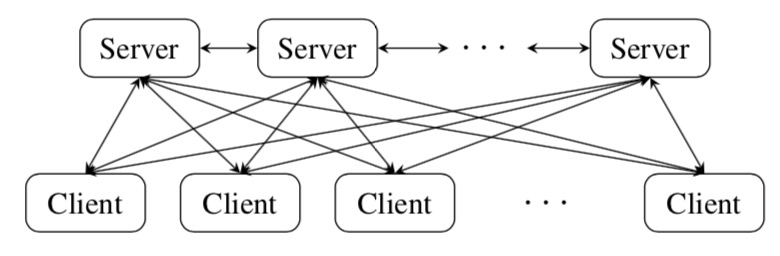
\includegraphics[width=10cm]{ps_comm_pattern}
\caption{参数服务器通信架构图}
\label{fig:ps_comm_pattern}
\end{figure}
参数服务器主要有5大优点:(1)通信高效,在异步情况下不会拖慢计算;(2)支持弹性一致性,其可通过放宽模型一致性条件,达到算法收敛速度和系统性能之间的平衡。(3) 扩展性强,增加节点时无需重启网络;(4)机器错误恢复时间短,Vector Clock容许网络错误了;(5)易用性,其全局共享的参数使用向量和矩阵表示,而这些又可以用高性能多线程库进行优化。

参数服务器下,训练流程如图~\ref{fig:ps_update_way}所示。训练主要包含4部分:(1)worker节点各自计算梯度;(2)worker节点将各自梯度push到server端;(3)server端对所有梯度进行求和平均并更新模型参数w;(4)worker节点从server端pull最新的参数w。

\begin{figure}[htp]
\centering
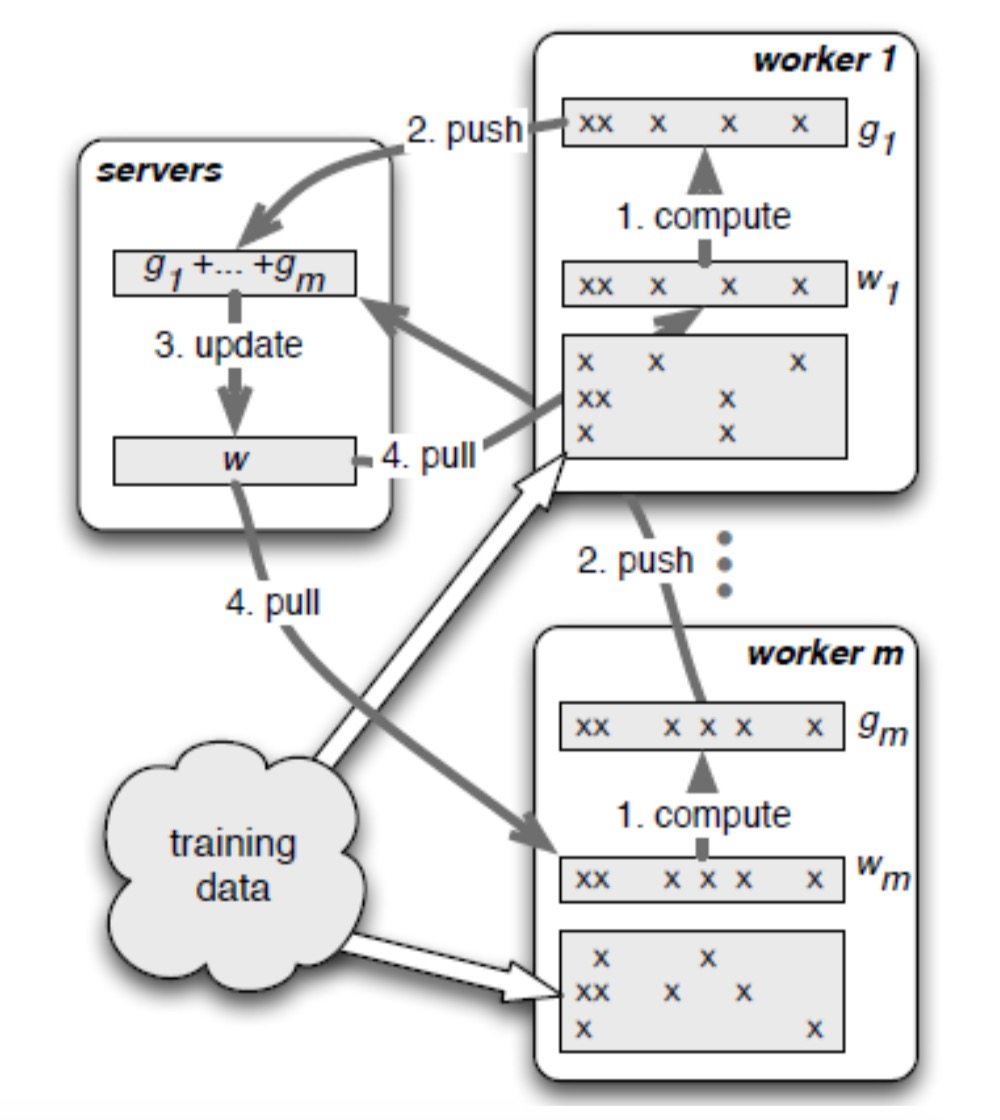
\includegraphics[width=11cm]{ps_update_way}
\caption{参数服务器下训练流程图}
\label{fig:ps_update_way}
\end{figure}
horovod\upcite{horovod2018}是uber基于百度ring-allredue的通信方式,提出了的分布式通信框架,因为其优异的性能和简单的使用方式,在业界引起广泛关注。horovod基于mpi实现,为提高分布式通信的效率,提出tensor fusion和分层级同步策略等方法,极大提高了分布式训练效率。 为方便用户查找分布式程序中的错误,分析程序性能等,其提供了Timeline监测工具,该工具可跟踪horovod中所有的事件,并以时间轴的形式展示,如图~\ref{fig:hvd_timeline_chrome}所示。极大简化了用户的分析工作,其为用户优化分布式程序性能提供了简单,有效的分析手段。
\begin{figure}[htp]
\centering
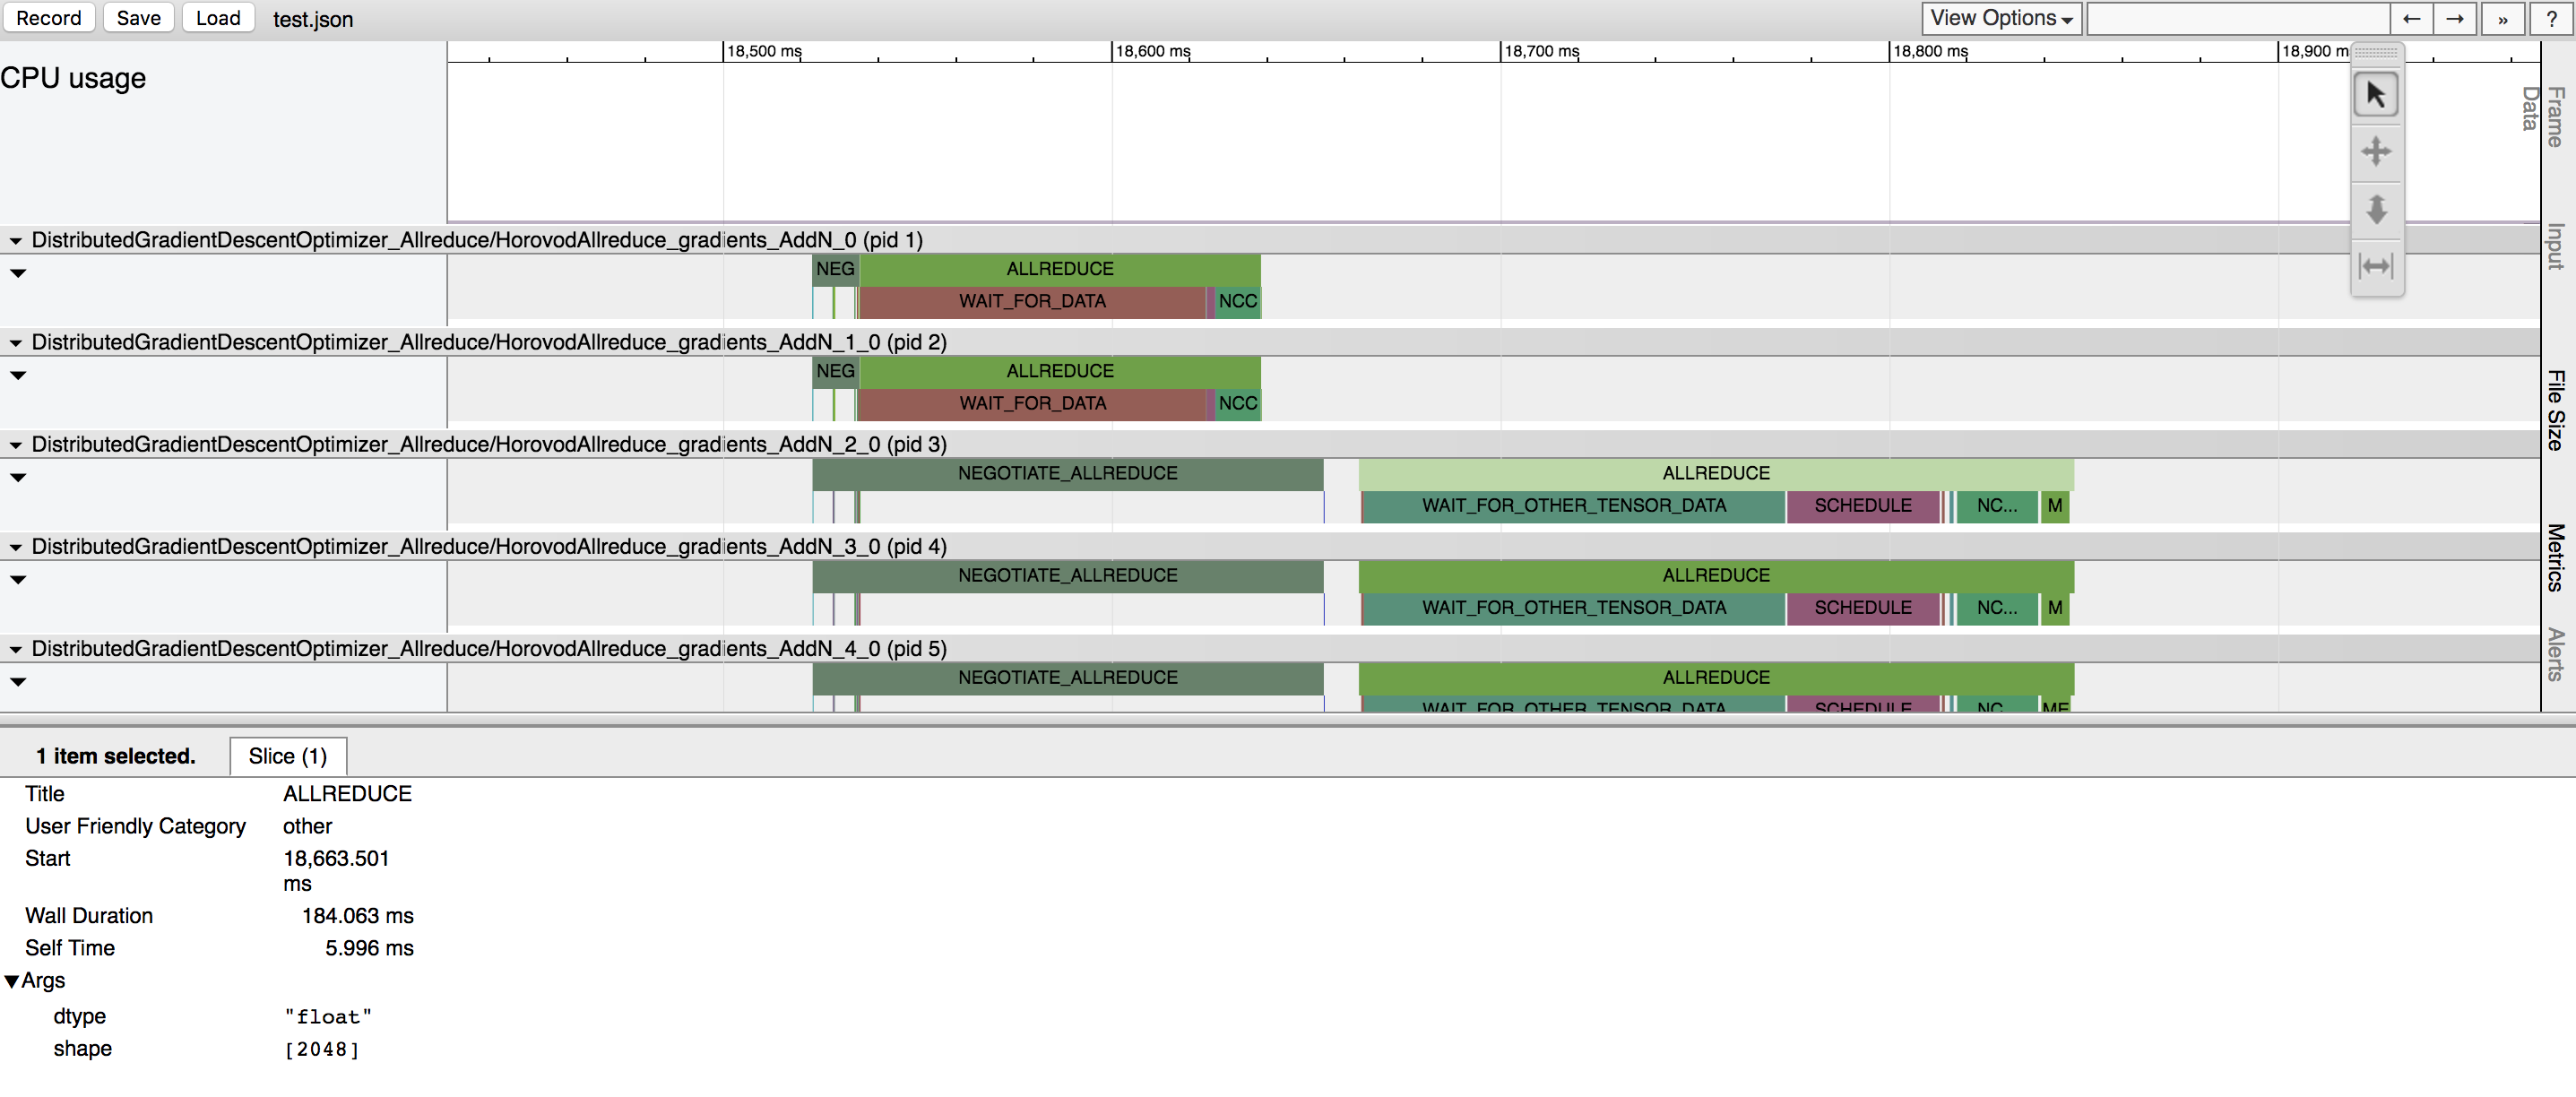
\includegraphics[width=13cm]{hvd_timeline_chrome}
\caption{chrome浏览器中timeline时刻表}
\label{fig:hvd_timeline_chrome}
\end{figure}

\subsection{低精度训练神经网络介绍}
因为传统硬件计算基本以浮点数为主,目前绝大多数训练场景中均采用浮点数计算。而神经网络本身存在随机性和容错性的特点,其计算精度并不需要达到浮点数的精度,为了节省内存,带宽,以及在支持低精度计算的硬件设备上提升计算效率,业界提出了两种主流的低精度数据格式用于神经网络训练。分别是IEEE半精度浮点数(FP16)和bfloat16(BF16)格式。两者与浮点数据格式区别如表~\ref{tab:diff_format_bits}所示。

\begin{table}[htbp]
\centering
\begin{minipage}[t]{0.9\linewidth}
\caption{不同数据格式比特位的详细分布}
\label{tab:diff_format_bits}
\begin{tabularx}{\linewidth}{l X X X X}
\toprule[1.5pt]
{\song 数据格式} & {\song 总比特位数} & {\song 符号位数} & {\song 指数位数} & {	\song 尾数位数}\\
\midrule[1pt]
FP32 & 32 & 1 & 8 & 23\\
FP16 & 16 & 1 & 5 & 10\\
BF16 & 16 & 1 & 8 & 7\\
\bottomrule[1.5pt]
\end{tabularx}
\end{minipage}
\end{table}
由科学计数法可知,表~\ref{tab:diff_format_bits}中3种数据格式在不同指数情况下,精度范围有所不同,3种数据格式所能表示的最小精度如表~\ref{tab:diff_format_precision}所示。经过工业界验证,用这两种数据格式训练神经网络均保证训练精度,逐渐成为主流。目前主流的深度学习框架tensorflow,pytorch,mxnet均支持半精度浮点数计算,BF16数据格式目前只有tensorflow针对自家硬件TPU有所支撑。

\begin{table}[htb]
\centering
\noindent\begin{minipage}{0.45\textwidth}
\centering
\caption{不同数据格式最小精度}
\label{tab:diff_format_precision}
\begin{tabular}{p{2cm}p{2cm}}
\toprule[1.5pt]
数据格式 & 数据精度 \\\midrule[1pt]
FP32 & 0.00000012 \\
FP16 & 0.00390625 \\
BF16 & 0.03125000 \\
\midrule[1pt]
\end{tabular}
\end{minipage}
\end{table}
2017年Micikevicius P等为节省训练的内存开销,提出混合精度训练\upcite{mixed2018}的方法,使用IEEE半精度格式存储所有网络层的中间结果。相对于原始32位浮点数计算而言,训练网络模型所消耗的内存减小了一半;同时,为了弥补半精度表示所带来的损失,文章提出混合精度更新方法,如图~\ref{fig:fp16_training_steps}所示。在设计损失函数时,适当放大损失函数权重的方法来保证训练精度。

\begin{figure}[htp]
\centering
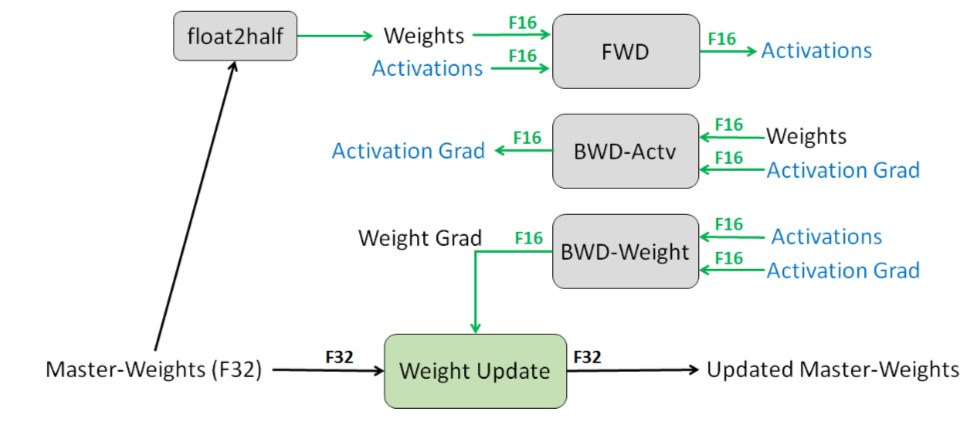
\includegraphics[width=13cm]{fp16_training_steps}
\caption{混合精度训练迭代方法}
\label{fig:fp16_training_steps}
\end{figure}
文章也指出,当前大部分硬件不支持半精度计算,所以此方法在现有硬件基础上只能节省内存,由于实际计算是先把半精度数值转换成浮点数再计算,存在一定的额外开销,使得计算速度相对有所下降。目前Nvidia的最新硬件,如Volta系列,turing系列已经支持半精度计算,可进一步提升计算效率。

受硬件条件和框架限制,只有Google公司将BF16数据格式用于训练神经网络,相关研究相对较少。根据其在ML perf\upcite{mlperf_result}中提交的相关结果可知,在图像分类、目标检测、自然语言处理等经典神经网络应用场景中BF16训练均能达到原始浮点数相同精度,证明了BF16数据格式用于神经网络训练的可行性和有效性。

\section{本文工作}
本课题旨在提高神经网络在分布式训练中的效率和分布式系统的可扩展性。根据目前业界对低精度数据在神经网络中的研究现状可知,BF16或FP16格式数据在一定优化方法下即可保证神经网络的精度。本课题提出低精度分布式更新(LPDU)算法,算法主要包含两部分:低精度通信和混合精度更新。算法核心思想是把原始浮点数梯度转换为BF16格式的低精度数据进行全局同步,使得同步数据量减半,进而减小同步时间开销,提高分布式训练效率。同时,为保证神经网络的训练精度,本文使用混合精度更新算法对神经网络进行更新。

在低精度分布式更新(LPDU)算法基础上,本文通过进一步减少梯度数据的有效尾数位继续减少同步数据量,以提升分布式训练系统的可扩展性和训练效率。结合半精度浮点数的数据格式,本文分别探索出两种极限精度梯度压缩(EPGC)方法:9比特梯度压缩方法和8比特梯度压缩方法。实验证明这两种压缩方法均能保证分类网的训练精度,证明了这两种压缩算法的可行性。

\subsection{低精度分布式更新算法}
BF16数据格式所需的数据位与半精度数据格式一致。其传输的数据量不变,而其指数位与浮点数一致,精度位比浮点数少了16位。相对于半精度数据而言有两个优势:1.在与浮点数进行转换的过程中,其与浮点数的转化更为高效。直接将浮点数的低16位舍去即可,无需对数据位进行转化;2.因为其指数位长度与浮点数一致,故其表示范围与浮点数基本一致,在进行数据转化时,不存在数值越界的情况。同时,因为BF16指数位相对较长,使得其精度位相对较短,其表示的精度相对半精度数据要差。

分布式训练相对于单机训练方式而言,仅多了同步梯度的过程,其同步开销大小决定了分布式训练效率的高低。考虑到现有硬件的特点和深度学习对低精度数据的友好性,本文提出使用浮点数据计算,BF16低精度数据通信,混合精度更新的训练方法。通过减少网络通信量的方法,提高分布式训练效率;使用混合精度更新的方法,保证神经网络精度与原始浮点数训练精度相一致。在LPDU算法下,神经网络在分布式更新过程中主要包含两部分:低精度通信和混合精度更新,具体设计与实验将在第三章详细介绍。

\subsection{极限精度梯度压缩方法}
考虑到梯度数据的特殊性:数值往往非常小,绝大部分梯度绝对值在0~1范围内。且随着训练过程中网络逐渐趋向于稳定,梯度数据的波动范围更小,更集中到0~1范围,可使用更少比特位表示梯度。通过减少梯度数据的表示位,可减少分布式训练程中的同步数据量,进而提高分布式系统的可扩展性和训练效率。

根据梯度数据这一特点,本文提出了专门用于针对梯度数据的两种极限精度梯度压缩(EPGC)方法:9比特压缩方法和8比特压缩方法,本文希望进一步减少梯度数据尾数位,探索在保证神经网络训练精度情况下梯度数据所需的最少比特位。为快速验证在特定尾数位情况下神经网络的训练精度,本文通过将原始浮点数或半精度浮点数特定尾数位清零的方法模拟特定比特位梯度压缩方法。经实验验证:在浮点数基础上仅保留2比特、1比特或去除所有尾数位均能保证分类网的训练精度。故本文提出去除所有尾数位的9比特(1个符号位,8个指数位)梯度压缩方法。结合半精度浮点数的特点,本文提出8比特梯度压缩方法:1个符号位,5个指数位,2个尾数位。实验证明该压缩算法同样能保证分类网的训练精度。具体设计与实验将在第四章详细介绍。

\section{本文组织结构}
本文针对现有硬件特点和神经网络对低精度数据的友好性,提出两种低精度数据传输方式,在保证训练精度的前提下,减小数据通信量,提升了分布式训练效率。文章主要探讨了在分布式训练神经网络中低精度数据传输的可行性以及不同数据表示的优劣点。本文主要分为五章,详细安排如下:

第一章,绪论。主要对本课题的研究背景和研究意义进行介绍,系统介绍了目前以神经网络为主的深度学习的发展,分布式深度学习系统的发展和低精度训练神经网络的最新进展以及现阶段计算硬件的限制。并说明了本文的主要研究内容以及对应的创新点。最后说明了本文的组织结构。

第二章,分布式训练神经网络和低精度训练的相关研究。首先介绍了分布式训练神经网络的基本概念,包括数据并行和模型并行两种典型并行方法;然后介绍了近年来神经网络在图像分类、目标检测、自然语言处理等领域的应用于发展;最后介绍了分布式深度学习的发展,包括分布式深度学习系统,优化算法和数据压缩等方面的研究进展。

第三章,低精度分布式更新算法。完整介绍了LPDU算法中低精度通信,混合精度更新算法的实现以及实验结果。首先介绍了将horovod整合进horovod中的实现方法;然后介绍了低精度高效通信算法和混合精度更新算法的设计与实现;最后具体介绍了相关实验内容,分析验证了低精度分布式更新算法在不影响神经网络训练精度的情况下对分布式训练效率的提升效果。

第四章,极限精度梯度压缩方法。分别介绍了两种梯度压缩方法:9比特梯度压缩方法与8比特梯度压缩方法。通过在浮点数或半精度浮点数基础上对特定尾数位置零的方法模拟这两种压缩方法。通过具体实验结果分析说明这两种梯度压缩方法的有效性。

第五章,总结与展望。对本课题的工作做出总结,说明本课题的两个创新点,指出基于目前研究进展未来需要做的下一步工作。
